\chapter{System Models and Control Requirements}
\section{Models}
A model of a system is a mathematical approximation of its behavior.

An input-output model of a systme is a set of equations that provide a nice estimation of the actual output values of the system within a certain range of input values.

\subsection{Operation point}
A continuous automated process operates at a specific woring point in order to comply wiht the production goal.

The working point is usually an equilibrium point of the system, which meand that all involved variables are constant over time (i.e. their derivatives are zero).

\subsection{Equilibrium point}
The variable values at the Equilibrium Point (equilibrium values) are usually denoted with a 0 subscript. SInce they are the final values when all the variables are kept constant, they are also referred to as the values when $t = \infty$.

Some equilibrium values must be known to determine the rest.


Broadly speaking, industrial processes are systems that present a non linear behavior. Even though there are serveral techniques to implement their control systems, this course will ofcus on the methods for linear incremental modeling around the so-called Equilibrium Point (E.P.)

In order to design and implement the control system of an industrial process we will need, first of all, a linear model around a certain equilibrium point.

The model may be obtained by meand of:
\begin{itemize}
    \item Linearizarion of differential equations
    \item Identification of actual systme behavior
\end{itemize}

\subsubsection{Linearization of a multi-input dynamical system}
Original system equations:
\[f(y, y', y'',..., u, u', u'',...) = 0\]
Nominal values:
\[y_0, y'_0, y''_0,..., u_0, u'_0, u''_0, ...\]
Linearized model
\[\frac{\partial f}{\partial y} \bigg|_0 \Delta y + \frac{\partial f}{\partial y'} \bigg|_0 \Delta y' + \frac{\partial f}{\partial y''} \bigg|_0 \Delta y'' + ... + \frac{\partial f}{\partial u} \bigg|_0 \Delta u + \frac{\partial f}{\partial u'} \bigg|_0 \Delta u' + \frac{\partial f}{\partial u''} \bigg|_0 \Delta u'' + ... = 0\]

The linear model is an incremental model
\begin{figure}[H]
    \centering
    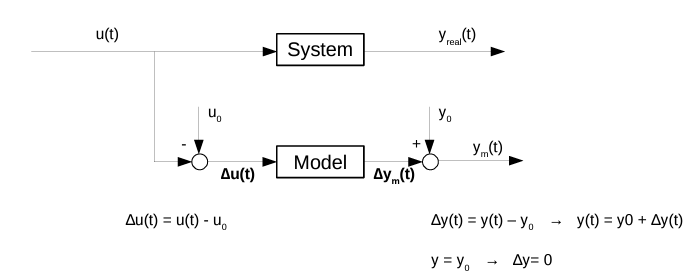
\includegraphics[width = 0.5 \textwidth]{Imagenes/2 - Linear Model.png}
    \label{Fig: 2 - Linear Model}
\end{figure}

The controller, the actuator, the transmitter, etc. are dynamical systems that we well model by means of differential equations.

In order to tune the controllers properly, transfer functions defined in the Laplace domain will be used instead of differential equations.

A transfer function is a linear model around a specific equilibrium point.

The linear approximation quality degrades as the variables get away from the selected equilibrium point.

\subsection{Linearization of a tank system}
In the following system:

a) Calculate the value for $h_0$ at the equilibrium point defined by $F_{10} = 1 m^3 / s$. Using Simulink, verify that this is an equilibrium point ($dh/dt = 0$)
\[dh/dt = 0 \rightarrow F_{i0} - 0.3 \sqrt{2 g h_0} = 0\]
\[h_0 = \frac{F_{i0}^2}{2ga^2}\]
\[F_{i0} = 1 \rightarrow h_0 = 0.5669\]

b) Obtain the liner model around this equilibrium point and calculate $H(s) / F_i(s)$
\[A \Delta \dot{h} = \Delta F_i (t) - \frac{a \sqrt{2g}}{2\sqrt{h}} \bigg|_0 \Delta h(t)\]
\[\Delta \dot{h}(t) + 0.882 \Delta h(t) = \Delta F_i (t) \]
\[\frac{H(s)}{F_1(s)} = \frac{1}{s + 0.882} = \frac{1.134}{1 + 1.134 s}\]

c) Obtain the new steady value $h_{0_2}$, both using the linear model and the non-linear model, when the flow grows 30\% form the previous equilibrium value ($F_{i0_2} = 1.3 m^3/s$)

\[ \Delta h (\infty) = \frac{\Delta F_i (\infty)}{0.0882} = \frac{F_{i02} - F_{i0}}{0.0882} = \frac{0.3}{0.882} = 0.34 \]

\[h_{linear}(\infty) = h_0 + \Delta h(\infty) = 0.5669 + \Delta h(\infty) = 0.907\]

\[h_{real}(\infty) = \frac{F_i^2(\infty)}{2ga^2} = \frac{1.3^2}{2 \cdot 9.8 \cdot 0.3^2} = 0.958\]

d) Using simulinkg, compare the evolution of $h(t)$ based on the linear model and the non-linear model, when the systems goes drom the equilibrium defined by $F_{i0} = 1$ to the new equilibrium point defined by $F_{i02} = 1.3$ (30\% variation) What about 10\% variation?

\begin{figure}[H]
    \centering
    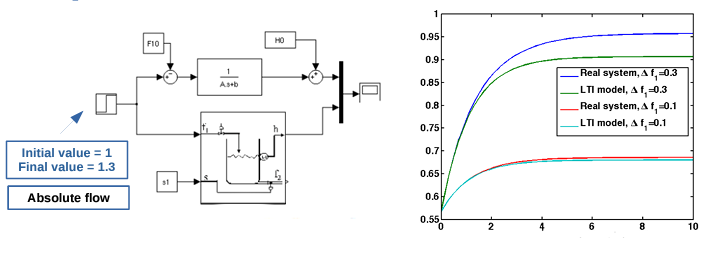
\includegraphics[width = 0.75 \textwidth]{Imagenes/2 - Linearization of a Tank System.png}
    \label{Fig: 2 - Linearization of a Tank System}
\end{figure}

The transfer funciton model is an incremental model. Hence the equilibrium values must always be added, as shown in the previous figures.

The linear model is an approximation of the real system. This is the reason why there is a difference between the exact new equilibrium value and the value porvided by the linear model.

\subsection{Modeling a valve}

\begin{figure}[H]
    \centering
    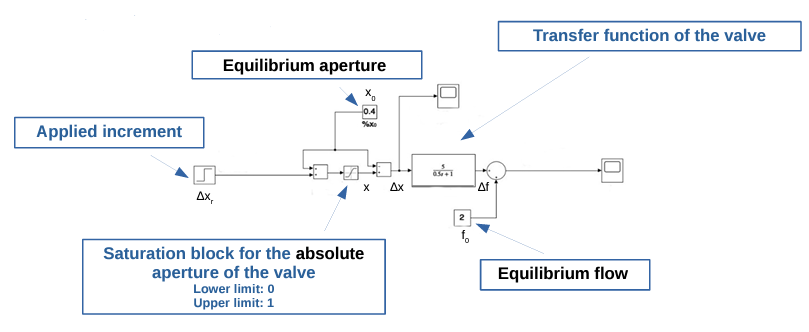
\includegraphics[width = 0.75 \textwidth]{Imagenes/2 - Modeling a Valve.png}
    \label{Fig: 2 - Modeling a Valve}
\end{figure}

How does a valve work?
\begin{itemize}
    \item The valve has an aperture range of $[0, 1]$
    \item The valve is initially opened a given \% of the maximum degree of aperture. This is the valve operation point (equilibrium point). E.g. the valve is initially 40\% opened.
    \item The valve aperture is modified a given \% from the operation point (opened or closed). If the valve is opened an additional 10\% then the valve is now 44\% opened ($0.4 + 0.04 = 0.44$)
    \item The new flow value from the valve is: the flow due to the increment (or reduction) of aperture from the operation point + the equilibrium flow.
    \item This is only true as long as the valve is not in a saturation state.
    \item The dynamical model of the valve, the transfer funciton Gv(s), is only used for the incremental opening or closing. The operation point flow $f_0$ (E.P) is always considered as a constant that must be added to the incremental flow obtained from the model of the valve. This is vary important.
\end{itemize}